\documentclass[runningheads]{llncs}
%

\usepackage[T1]{fontenc}
\usepackage{amsmath,amssymb,amsfonts}
\usepackage{subcaption}
\usepackage{graphicx}
% Used for displaying a sample figure. If possible, figure files should
% be included in EPS format.
%
% If you use the hyperref package, please uncomment the following two lines
% to display URLs in blue roman font according to Springer's eBook style:
%\usepackage{color}
%\renewcommand\UrlFont{\color{blue}\rmfamily}
%\urlstyle{rm}
%
\begin{document}
%
%\title{Robust Automatic Modulation Classification via Heterogeneous Deep Ensemble Learning}
\title{MF-SR-OCR: End-to-End Joint Multi-Frame Super-Resolution and Recognition for Low-Resolution License Plate}
%
\titlerunning{MF-SR-OCR for Low-Resolution License Plate Recognition}
% If the paper title is too long for the running head, you can set
% an abbreviated paper title here
%
\author{Nhut-Minh Nguyen\inst{1,4} and 
Vo-Trung-Dung Huynh\inst{2,3,5}\orcidID{0000-0002-9678-8335} 
}
%
\authorrunning{Nhut-Minh Nguyen et al.}
% First names are abbreviated in the running head.
% If there are more than two authors, 'et al.' is used.
%
\institute{FPT School of Business and Technology, Ho Chi Minh City, Vietnam \and
International University, VNU-HCM, Ho Chi Minh City, Vietnam \and
Viet Nam National University Ho Chi Minh City, Vietnam \and
\email{minhnn25ms23283@fpt.edu.vn} \and 
\email{hvtdung@hcmiu.edu.vn}
}
%
\maketitle              % typeset the header of the contribution
%
\begin{abstract}
Low-Resolution License Plate Recognition (LRLPR) remains a critical challenge in surveillance due to severe motion blur, long capture distances, and lossy video compression. While traditional pipelines treat image restoration and character recognition as decoupled stages, this work investigates the synergy of end-to-end joint optimization. We introduce MF-SR-OCR, a unified Multi-Frame Super-Resolution and Recognition framework tailored for low-resolution video tracks. The proposed architecture integrates per-frame Spatial Transformer Network (STN) alignment, deformable (DCNv2) cross-frame feature alignment, pixel-supervised super-resolution, attention-guided multi-frame fusion, and layout-constrained Connectionist Temporal Classification (CTC) decoding, optimized jointly using Exponential Moving Average (EMA) weight smoothing. Systematic ablation isolates the contributions of a GroupNorm-stabilized ResBlock backbone and pixel-level restoration against a multi-frame CRNN+STN baseline. Evaluated on authentic surveillance tracks, MF-SR-OCR consistently outperforms all baseline variants beyond the validation noise floor. Crucially, the learned super-resolution branch maintains a reconstruction loss significantly below bilinear interpolation baselines throughout training, demonstrating genuine sub-pixel detail recovery rather than cosmetic smoothing. Our findings validate joint restoration-recognition optimization for unconstrained LRLPR and highlight the critical necessity of multi-seed evaluation when benchmarking subtle architectural iterations.
\keywords{license plate recognition \and low-resolution image \and super resolution \and spatial transformer network \and multi-frame fusion.}
\end{abstract}
%
%
%
\section{Introduction}

Automatic License Plate Recognition (ALPR) has reached near-saturation accuracy on well-resolved imagery, where modern detectors and sequence recognizers resolve plate characters almost perfectly \cite{laroca2018robust,laroca2022cross}. Operational surveillance, however, violates the assumptions behind those results: plates are captured at long standoff distances with limited sensor resolution, corrupted by motion blur, and further degraded by lossy video compression. Under such conditions the character stroke width collapses to a small number of pixels, and recognition rates fall by an order of magnitude \cite{nascimento2025toward}. Low-Resolution License Plate Recognition (LRLPR) has consequently emerged as a distinct problem, formalized by a recent large-scale international benchmark built on authentic—rather than synthetically downsampled—degraded tracks, where the winning entry attains only $82.13\%$ recognition rate, confirming that the task remains unsolved \cite{laroca2026icpr}.

The dominant response to this degradation is to insert a super-resolution (SR) stage before recognition. Generic SR backbones, from early convolutional regressors \cite{dong2016srcnn} and sub-pixel convolution \cite{shi2016espcn} to transformer-based restorers \cite{liang2021swinir}, optimize pixel fidelity over natural images and are therefore poorly matched to the thin, high-frequency glyph structures that determine plate legibility. Plate-specific designs narrow this gap by injecting attention and pixel-shuffle upsampling \cite{nascimento2022combining,nascimento2023attention}, layout and character priors \cite{nascimento2024lcdnet}, or embedding-level consistency between high-resolution and super-resolved plates \cite{sendjasni2025embedding}; the analogous trend in scene-text SR replaces synthetic degradation with real paired captures \cite{wang2020textzoom}. Two limitations persist across this line of work. First, restoration and recognition are trained as \emph{decoupled} stages, so the SR objective optimizes a perceptual or pixel criterion that correlates weakly with downstream OCR accuracy—an effect documented explicitly for license plates, where PSNR and SSIM fail to track recognition performance \cite{tsai2025deep,nascimento2025toward}. Second, generative restorers driven by pretrained priors can hallucinate plausible but incorrect glyphs, which is unacceptable when the output serves as forensic evidence \cite{na2025mflpr2}.

A complementary source of information is temporal redundancy: surveillance systems observe each vehicle over a short track rather than a single frame, and independent noise and sub-pixel sampling offsets across frames carry detail that no single-image restorer can recover. Multi-frame fusion is now standard in video restoration, whether through deformable alignment \cite{zhu2019dcnv2,wang2019edvr} or recurrent propagation \cite{chan2021basicvsr}, and its benefit for plates is pronounced: majority-vote fusion over five super-resolved frames raises recognition from $31.1\%$ to $44.7\%$ \cite{nascimento2025toward}, while optical-flow-based multi-frame restoration lifts accuracy from $14.04\%$ for the best single-frame model to $86.44\%$ \cite{na2025mflpr2}. These systems nevertheless still fuse in pixel space and hand the result to a frozen recognizer, leaving the restoration objective blind to the recognition loss.

This work investigates whether closing that loop pays off. We introduce MF-SR-OCR, a unified framework in which per-frame geometric rectification via a Spatial Transformer Network \cite{jaderberg2015stn}, deformable cross-frame feature alignment \cite{zhu2019dcnv2}, pixel-supervised super-resolution, attention-guided multi-frame fusion, and layout-constrained CTC decoding \cite{graves2006ctc} over a CRNN recognition head \cite{shi2017crnn} are optimized jointly under a single objective, stabilized by a GroupNorm-based backbone \cite{wu2018groupnorm} and Exponential Moving Average weight smoothing \cite{tarvainen2017mean}. Systematic ablation isolates the contribution of each component against a multi-frame CRNN+STN baseline on authentic surveillance tracks \cite{laroca2026icpr}. Our contributions are threefold: (i) an end-to-end architecture that lets the recognition loss shape the restoration branch instead of treating SR as fixed preprocessing; (ii) evidence that the learned SR branch sustains a reconstruction loss well below bilinear interpolation throughout training, indicating genuine sub-pixel recovery rather than cosmetic smoothing; and (iii) a multi-seed evaluation protocol quantifying the validation noise floor, without which the small margins reported between competing LRLPR variants cannot be distinguished from run-to-run variance. The remainder of this paper is organized as follows. Section~2 details the proposed architecture and training objective, Section~3 presents the experimental setup and results, and Section~4 concludes the work.


%%%%%%%%%%%%%%%%%%%%%%%%%%%%%%%%%%%%%%%%%%%%%%%%%%%%%%%%%%%%%%%%%%%%%%%%%%%%%%%%%%%%%%%%

\section{Methodology}

This section delineates the architectural and procedural framework of the proposed SNR-adaptive AMC system. We first formalize the signal propagation model and the stochastic channel impairments utilized for dataset synthesis. Subsequently, we detail the preprocessing pipeline—specifically the transformation of complex baseband signals into eye diagrams—and conclude with the specific layer configurations of the heterogeneous neural network ensemble.

%%%%%%%%%%%%%%%%%%%%%%%%%%%%%%%%%%%%%%%%%%%%%%%%%%%%%%%%%%%%%%%%%%%%%%%%%%%%%%%%%%%%%%%%

\subsection{Signal Propagation Model and Dataset Synthesis}

The data acquisition framework implements a rigorous, multi-stage generation protocol designed to synthesize a comprehensive signal taxonomy comprising 11 distinct modulation schemes—spanning eight digital formats\footnote{BPSK, QPSK, 8-PSK, 4-PAM, 16-QAM, 64-QAM, GFSK, CPFSK.} and three analog waveforms\footnote{AM-DSB, AM-SSB, WBFM.}—transmitted over a synthetic channel engineered to emulate stochastic Non-Line-of-Sight (NLOS) urban propagation dynamics. The simulation model explicitly incorporates Rayleigh multipath fading (parameterized by path delays $\tau = [0, 0.9, 1.7]$ samples and attenuation gains $\alpha = [0, -2, -10]$ dB) and Additive White Gaussian Noise (AWGN) sweeping a dynamic range of $-20$ dB to $18$ dB, further compounded by random frequency and phase offsets (capped at $0.01$ radians) to account for hardware synchronization artifacts. To capture temporal signal integrity and inter-symbol interference (ISI), these raw waveforms are transformed into eye diagram representations—formalized as a tensor spanning $M$ modulation classes and $N$ independent frames of length $N_s$—and subsequently decomposed into orthogonal In-phase ($I$) and Quadrature ($Q$) channels. Critically, to prevent the deep learning architecture from overfitting to non-informative graphical constraints, an automated Region of Interest (ROI) extraction process excises deterministic artifacts (e.g., axes and grids), ensuring generalization is based exclusively on signal morphology. This extensive pipeline yields a high-density corpus of $1.28 \times 10^6$ frames per modulation-SNR pair, culminating in a total dataset volume of $5.63 \times 10^8$ frames; to facilitate unbiased benchmarking, this data is finally stratified into training ($70\%$), validation ($15\%$), and testing ($15\%$) subsets, providing a statistically significant foundation for evaluating inference accuracy across diverse noise regimes.

%%%%%%%%%%%%%%%%%%%%%%%%%%%%%%%%%%%%%%%%%%%%%%%%%%%%%%%%%%%%%%%%%%%%%%%%%%%%%%%%%%%%%%%%

\subsection{Heterogeneous Deep Ensemble Learning Architecture}

\begin{figure}[!h]
    \centering
    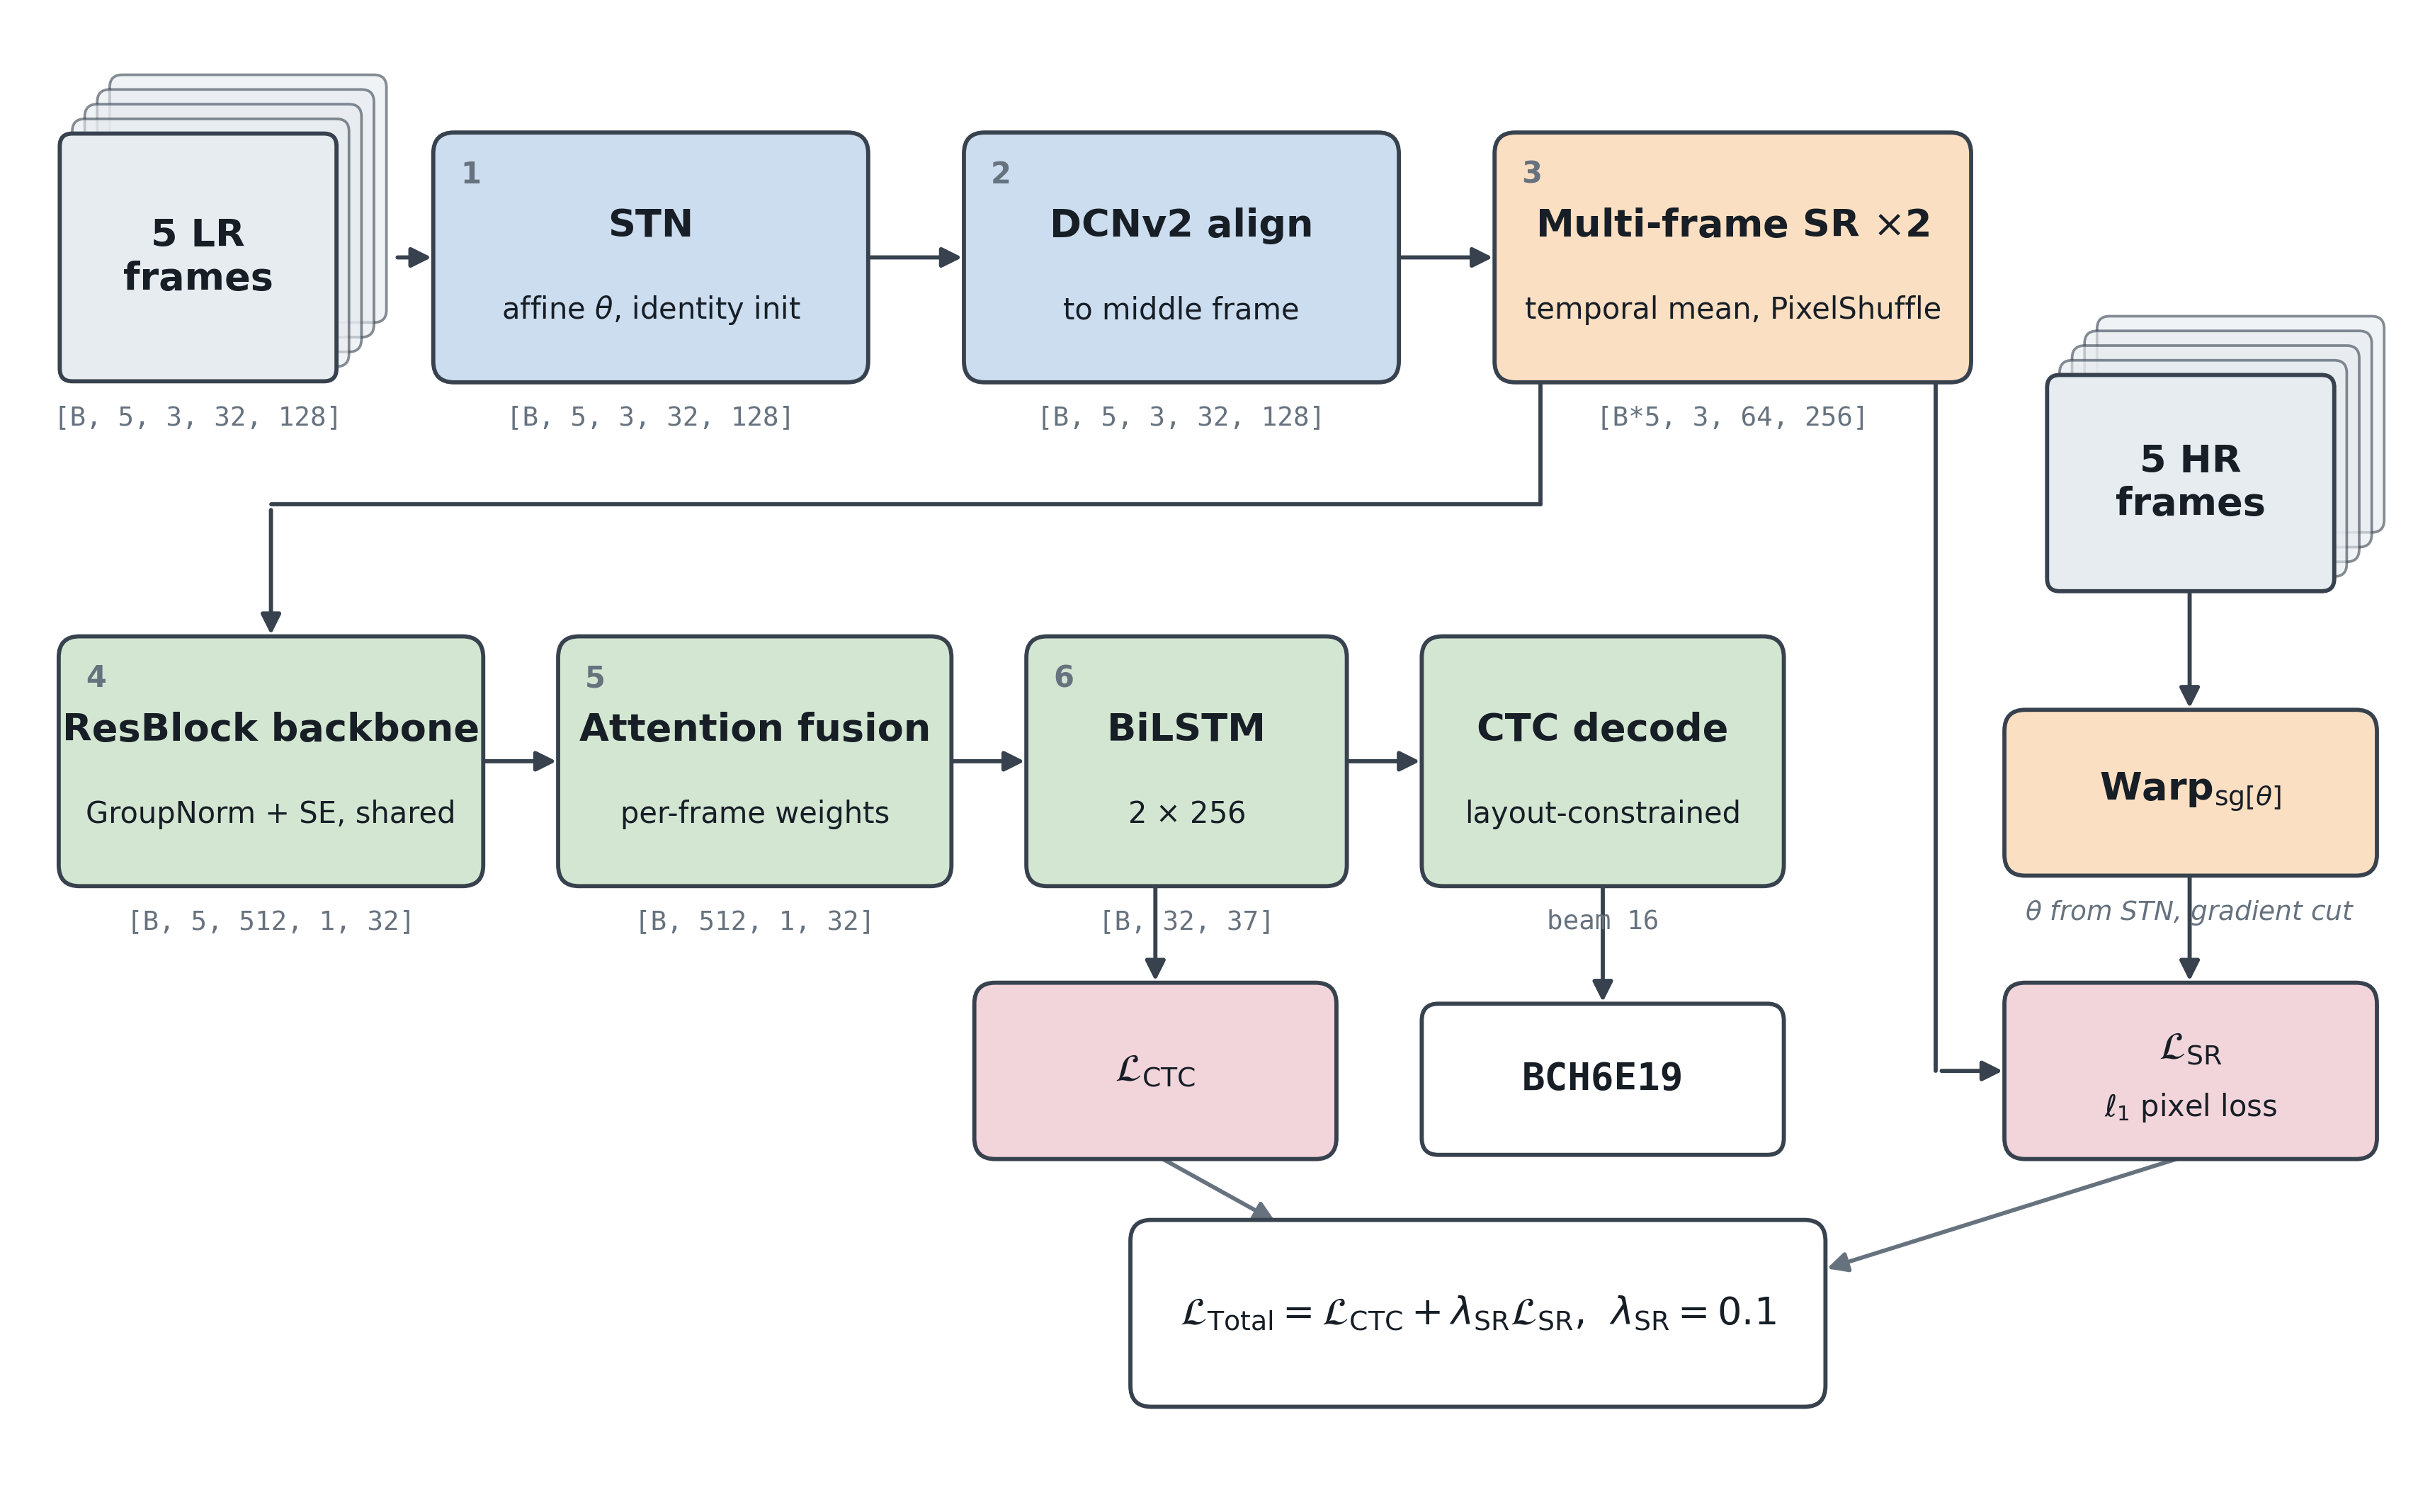
\includegraphics[width=1\textwidth,  height = 0.4\textheight, keepaspectratio]{Methonology/SystemOverview.png}
    \caption{Heterogeneous deep ensemble learning architecture with adaptive gating.}
    \label{fig1}
\end{figure}

The proposed Automatic Modulation Classification (AMC) framework functions as an end-to-end, SNR-adaptive deep learning ecosystem designed to map raw $I/Q$ signal representations directly to modulation probability distributions. Departing from conventional monolithic architectures that typically exhibit limited generalization across dynamic fading channels, this study implements a regime-aware heterogeneous ensemble strategy that orchestrates a bank of complementary neural feature extractors optimized for distinct signal integrity zones. Specifically, the architecture synergizes a Transformer Neural Network (TNN), leveraging self-attention mechanisms to model robust global dependencies in noise-dominated environments where local signal morphology is heavily corrupted, with high-fidelity Convolutional specialists (Shallow ResNet or CLDNN) engineered to resolve fine-grained spatial hierarchies in complex constellations (e.g., high-order QAM) when signal structure is preserved.

To ensure the system's reliability and interpretability, the SNR Estimator is implemented using the blind $M_2M_4$ statistical moment-based estimator. This method is selected for its computational efficiency and independence from modulation types, making it suitable for blind classification tasks. The estimator calculates the second and fourth-order moments of the received signal $y(n)$ to derive the estimated SNR, $\hat{\gamma}$. The estimated SNR governs the ensemble aggregation through a dynamic gating mechanism. Unlike static averaging, we employ a soft-gating strategy where the final predicted probability vector $\hat{\mathbf{y}}$ is a weighted fusion of the TNN and CNN outputs ($z_{TNN}$ and $z_{CNN}$):
\begin{equation}
    \hat{\mathbf{y}} = \sigma \left( \lambda_{TNN}(\hat{\gamma}) \cdot \mathbf{z}_{TNN} + \lambda_{CNN}(\hat{\gamma}) \cdot \mathbf{z}_{CNN} \right),
\end{equation}
where $\sigma(\cdot)$ denotes the Softmax activation function. The weighting coefficients $\lambda(\hat{\gamma})$ are determined by a logistic sigmoid function centered at a learnable threshold $\gamma_{th}$:
\begin{equation}
    \lambda_{CNN}(\hat{\gamma}) = \frac{1}{1 + e^{-k(\hat{\gamma} - \gamma_{th})}}, \quad \lambda_{TNN}(\hat{\gamma}) = 1 - \lambda_{CNN}(\hat{\gamma}).
\end{equation}
In this study, the gating threshold is empirically set at $\gamma_{th} = 0 \text{ dB}$ with a scaling factor $k=10$ to approximate a hard-switching behavior while maintaining differentiability. This design choice is validated by the "waterfall" performance breakdown observed in our validation set: the TNN's global self-attention provides a stabilizing gain of approximately $12\%$ over convolutional baselines in the Noise-Dominated Regime ($\hat{\gamma} < 0 \text{ dB}$), whereas the ResNet/CLDNN streams dominate in feature spatiality for the Signal-Dominated Regime ($\hat{\gamma} \ge 0 \text{ dB}$), maximizing the separation of dense modulation schemes.


%%%%%%%%%%%%%%%%%%%%%%%%%%%%%%%%%%%%%%%%%%%%%%%%%%%%%%%%%%%%%%%%%%%%%%%%%%%%%%%%%%%%%%%%

\subsection{Deep Learning Models}

To realize the heterogeneous deep ensemble architecture depicted in Fig. \ref{fig1}, this study prioritizes the development and rigorous optimization of three complementary neural backbones. The objective is to maximize modulation classification accuracy through the strategic integration of distinct feature extraction paradigms. Specifically, the ensemble aggregates the following Deep Neural Network (DNN) architectures, each fine-tuned via extensive hyperparameter optimization:

%%%%%%%%%%%%%%%%%%%%%%%%%%%%%%%%%%%%%%%%%%%%%%%%%%%%%%%%%%%%%%%%%%%%%%%%%%%%%%%%%%%%%%%%

\textbf{Shallow Resnet Model}: The proposed backbone employs a modified ResNet architecture utilizing Bottleneck Residual Units ($1\times1$ compression, $3\times3$ extraction, $1\times1$ expansion). Raw $128 \times 2$ I/Q sequences are processed by a Stem Layer (Conv1D, $k=7, s=2$) followed by three stages expanding feature depth from 256 to 1024 (internal widths: 64, 128, 256). The hierarchy integrates Identity Blocks ($x + \mathcal{F}(x)$) for aligned dimensions and Convolutional Blocks with strided shortcuts for downsampling. Finally, Global Average Pooling (GAP) condenses the output for a classification head consisting of Dropout ($p=0.5$), a 128-unit dense layer, and Softmax activation.

% \begin{figure}[h]
%     \centering
%     \includegraphics[width=1\textwidth]{Methonology/Identity and Conv of Resnet.png}
%     \caption{Identity Block and Conv Block}
%     \label{fig:Identity and Conv}
% \end{figure}

% \begin{figure}[!h]
%     \centering
%     \includegraphics[width=1\textwidth]{Methonology/Shallow Resnet.png}
%     \caption{Shallow Resnet Model}
%     \label{fig:Shallow Resnet Model}
% \end{figure}

%%%%%%%%%%%%%%%%%%%%%%%%%%%%%%%%%%%%%%%%%%%%%%%%%%%%%%%%%%%%%%%%%%%%%%%%%%%%%%%%%%%%%%%%

\textbf{Convolutional Long-Short Term Deep Neural Network Model}: Functioning as a spatiotemporal complement, the Hybrid CLDNN retains the Bottleneck Residual backbone but replaces Global Average Pooling with a sequence-preserving mechanism, yielding a latent tensor of shape $(16, 1024)$. This sequence is processed by a 128-unit Gated Recurrent Unit (GRU)—selected over LSTM for superior parameter efficiency and convergence—to aggregate temporal dependencies. The resulting 128-dimensional context vector feeds into a classification head comprising a 128-unit ReLU dense layer flanked by dual Dropout layers ($p=0.5$) and a terminal Softmax activation.

% \begin{figure}[h]
%     \centering
%     \includegraphics[width=1\textwidth]{Methonology/CLDNN.png}
%     \caption{CLDNN Model}
%     \label{fig:CLDNN Model}
% \end{figure}

%%%%%%%%%%%%%%%%%%%%%%%%%%%%%%%%%%%%%%%%%%%%%%%%%%%%%%%%%%%%%%%%%%%%%%%%%%%%%%%%%%%%%%%%

\textbf{Transformer Neural Network Model}: The third branch employs a Transformer Neural Network (TNN) to capture global temporal dependencies. A Convolutional Tokenization Stem (Conv1D, Max Pooling) projects the raw $128$-sample input into $64$ feature tokens, augmented by Learnable Positional Embeddings to enforce sequence order. The core architecture comprises a stack of $L=8$ Transformer Encoder blocks, each integrating Multi-Head Self-Attention ($H=8$) and a $128$-unit Position-wise Feed-Forward Network (FFN), stabilized via residual connections ($x + \text{Sublayer}(x)$) and Layer Normalization. The output is condensed via Global Average Pooling (GAP) and processed by a classification head consisting of a $128$-unit ReLU dense layer, Dropout ($p=0.1$), and Softmax activation.


% \begin{figure}[h]
%     \centering
%     \includegraphics[width=1\textwidth]{Methonology/Token and Pos.png}
%     \caption{Token and Position Embedding Block}
%     \label{fig:Token and Position Embedding Block}
% \end{figure}

% \begin{figure}[h]
%     \centering
%     \includegraphics[width=1\textwidth]{Methonology/TNN Model.png}
%     \caption{TNN Model}
%     \label{fig:TNN Model}
% \end{figure}

%%%%%%%%%%%%%%%%%%%%%%%%%%%%%%%%%%%%%%%%%%%%%%%%%%%%%%%%%%%%%%%%%%%%%%%%%%%%%%%%%%%%%%%%

\section{Numerical Results and Discussion}




To ensure experimental consistency and reproducibility, a unified hyperparameter configuration was enforced across all candidate architectures. The models were implemented within the TensorFlow deep learning framework. Network weights were optimized using the Adam algorithm with a static learning rate of $\alpha = 5 \times 10^{-4}$. This specific learning rate was empirically selected to balance convergence speed with stability, effectively mitigating the gradient volatility often observed in the recurrent units of the CLDNN and the multi-head attention blocks of the TNN. The loss calculation utilized Sparse Categorical Cross-Entropy, minimizing the divergence between the predicted probability distribution and the ground-truth modulation labels. Further, the performance analysis assesses classification accuracy across a wide dynamic range of signal-to-noise ratios (SNRs), i.e., from $-20$ dB to $+20$ dB. 

\begin{figure}[h]
    \centering
    \includegraphics[width=1\textwidth,  height = 0.4\textheight, keepaspectratio]{Result/Ensemble.png}
    \caption{Accuracy vs. SNR of different techniques.}
    \label{fig2}
\end{figure}

Fig. \ref{fig2} delineates the definitive performance benchmark, wherein the heterogeneous fusion of the Shallow ResNet and TNN (solid red trajectory) establishes a dominant operational envelope across the full dynamic range, peaking at an asymptotic accuracy of $\approx 94\%$ in the high-SNR regime ($> 10\,\text{dB}$) while demonstrating superior gradient stability in the critical transition zone ($0\text{--}4\,\text{dB}$). This empirical success validates the hypothesis of feature orthogonality: the architecture effectively synergizes the high-precision spatial filtering of the ResNet—essential for resolving dense, static constellations (e.g., 64-QAM)—with the global, noise-resilient context of the TNN, thereby rectifying errors in noise-dominated samples where local convolutional filters lose discriminative power and yielding a calibrated, robust classification output. In stark contrast, the CLDNN-TNN configuration yields suboptimal inference results (saturating at $90\%\text{--}91\%$) due to feature redundancy and overlapping inductive biases; since both constituent architectures (via recurrent units and self-attention, respectively) are predisposed toward extracting temporal dependencies, they exhibit correlated error manifolds—particularly in differentiating high-order memoryless modulations like 64-QAM vs. 8-PSK—resulting in a compounded "temporal bias" that fails to provide the requisite diversity needed for effective ensembling.

\begin{figure}[!h]
    \centering
    \includegraphics[width=1\textwidth, height = 0.4\textheight, keepaspectratio]{Result/CM Resnet TNN.png}
    \caption{Confusion Matrix of Ensembling Shallow Resnet and TNN.}
    \label{fig3}
\end{figure}

\begin{figure}[!h]
    \centering
    \includegraphics[width=1\textwidth, height = 0.4\textheight, keepaspectratio]{Result/CM CLDNN TNN.png}
    \caption{Confusion Matrix of Ensembling CLDNN and TNN.}
    \label{fig4}
\end{figure}

The confusion matrix presented in Fig. \ref{fig3} delineates the system's performance within the critical "Transition Regime" ($\text{SNR} \approx 0\,\text{dB}$), where the ensemble demonstrates a strategic fusion of spatial rigidity and contextual resilience. Notably, the architecture achieves exceptional fidelity in analog domains—recording $93\%$ accuracy for Wideband Frequency Modulation (WBFM) and exceeding $73\%$ for Amplitude Modulation schemes—a result we attribute to the Transformer's global attention mechanism acting as a "spectral validator" that filters spurious local correlations and eliminates the false-positive mode collapse frequently observed in standalone convolutional baselines. While discrimination in dense digital constellations (e.g., QAM, PSK) is naturally bounded between $48\%$ and $60\%$ by the noise-obscured Euclidean distances, the ensemble maintains strict Manifold Preservation: errors are not stochastic but are statistically clustered among spectrally adjacent sub-classes (e.g., misclassifying 64-QAM as 16-QAM). This structured error distribution confirms that the heterogeneous fusion preserves the topological integrity of the modulation space, preventing catastrophic classification bias even when the noise floor challenges definitive symbol discrimination.

To isolate the specific contribution of deep residual spatial filtering, we evaluate the CLDNN-Transformer ensemble, where the performance dynamics reveal a stark divergence contingent on modulation topology. While the classification of continuous analog waveforms remains robust—virtually invariant to the backbone choice due to the Transformer's dominance in resolving global temporal envelopes (matching the 93\% WBFM benchmark of the ResNet-based system)—the digital domain suffers a precipitous degradation in fidelity. Specifically, 16-QAM detection collapses to 39\% (a 9\% deficit relative to the ResNet-TNN benchmark), with concomitant losses across phase-dependent schemes like 8PSK and QPSK. We attribute this sub-optimal performance to feature redundancy and a compound spatial deficit: the CLDNN’s reliance on recurrent aggregation functionally overlaps with the Transformer’s self-attention mechanism, resulting in an ensemble with correlated temporal inductive biases but insufficient spatial resolution. Lacking the deep residual regularization provided by the ResNet to disentangle dense Euclidean clusters, the framework fails to enforce the precise decision boundaries required for high-order memoryless modulations, confirming that rigorous spatial feature extraction is a non-negotiable prerequisite for robust digital signal separation.

%%%%%%%%%%%%%%%%%%%%%%%%%%%%%%%%%%%%%%%%%%%%%%%%%%%%%%%%%%%%%%%%%%%%%%%%%%%%%%%%%%%%%%%%
\section{Conclusion}

This study advances AMC robustness in stochastic NLOS environments by proposing an SNR-adaptive heterogeneous ensemble that strategically fuses Shallow ResNet spatial filtering with Transformer-based global attention. The primary contribution lies in the exploitation of feature orthogonality to stabilize the decision boundary: the framework leverages ResNet precision to resolve dense constellations in signal-dominated regimes, while uniquely deploying the Transformer as a spectral validator to prevent mode collapse in noise-dominated zones, thereby achieving $\approx 94\%$ asymptotic accuracy. By empirically invalidating redundant spatiotemporal combinations (e.g., CLDNN-TNN), this work confirms that strict architectural diversity is the prerequisite for effective ensembling, establishing a validated foundation for future edge-native, Over-The-Air implementations.


%%%%%%%%%%%%%%%%%%%%%%%%%%%%%%%%%%%%%%%%%%%%%%%%%%%%%%%%%%%%%%%%%%%%%%%%%%%%%%%%%%%%%%%%
\bibliographystyle{IEEEtran}
\bibliography{refs}

\end{document}
